\section{Analyzing Agent Performance}

% 1
\subsection{What is the relation b/w the improvement in terms of Pareto Rate vs the cost of running the agent?}

\begin{figure}[t]
    \centering
    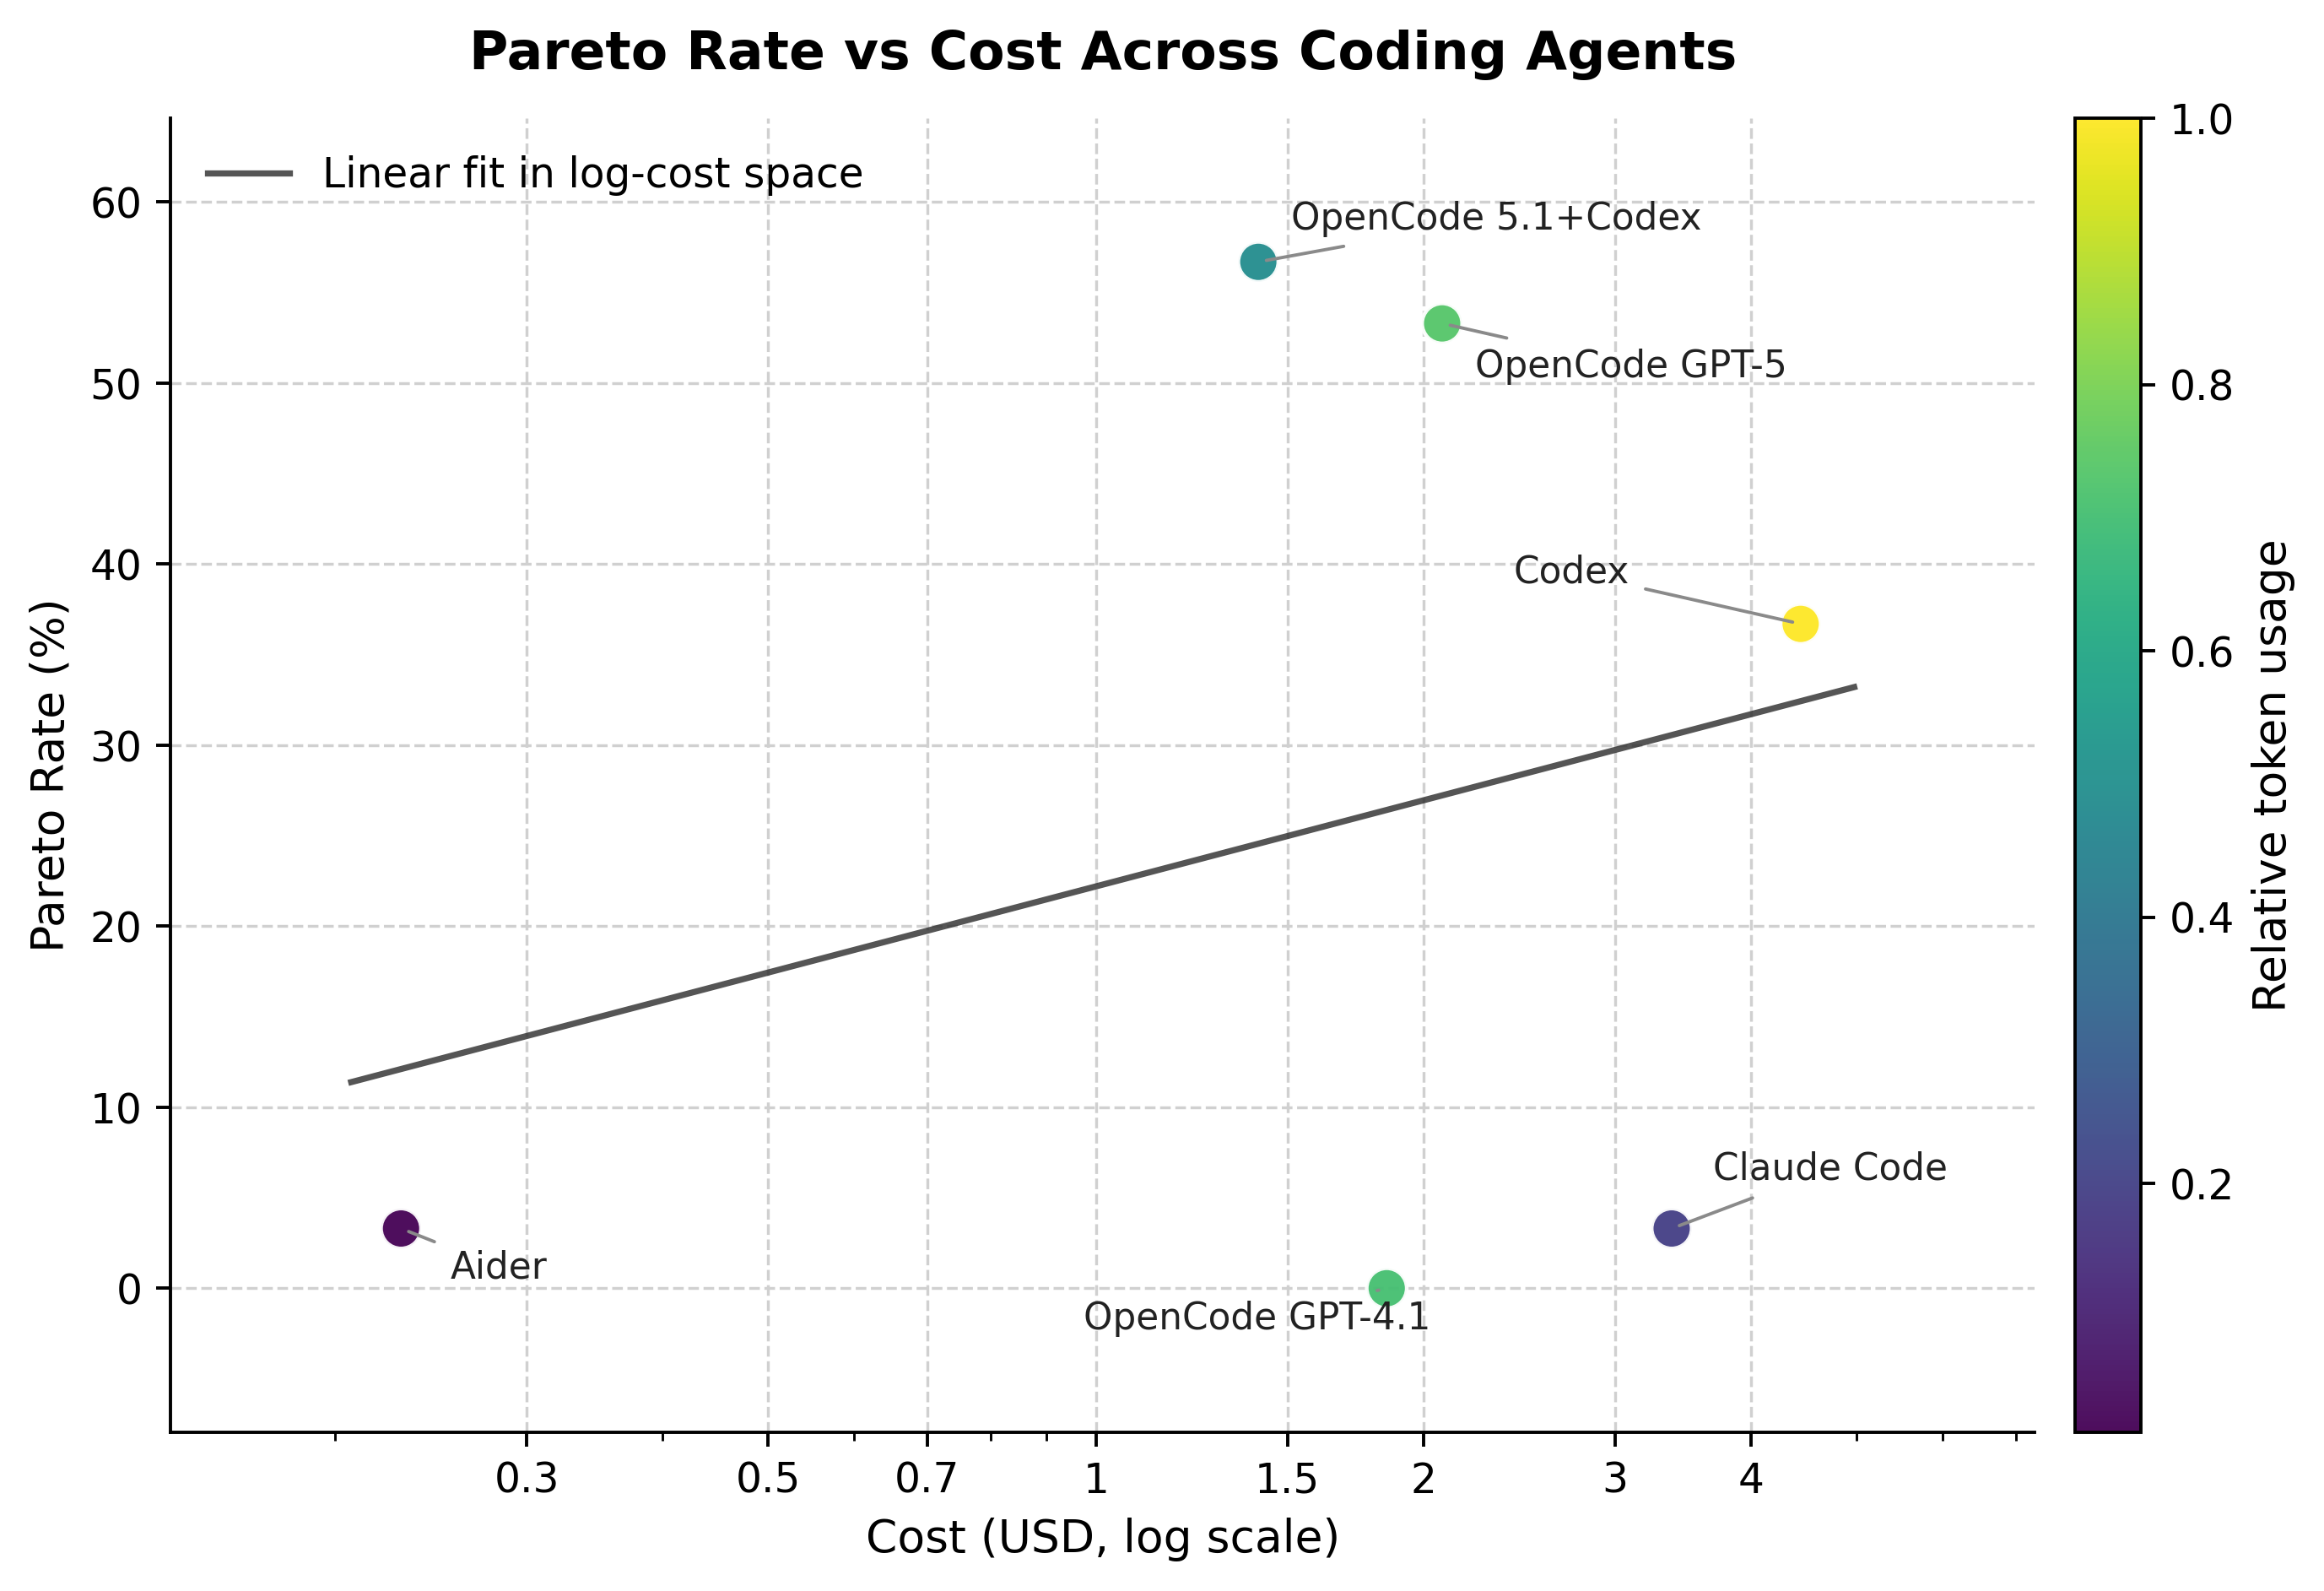
\includegraphics[width=0.7\linewidth]{figures/fig_pareto_rate_vs_cost.png}
    \caption{Pareto Rate Improvement vs Cost / Token usage across agents.}
    \label{fig:cost_tokens}
\end{figure}

% 2
\subsection{Which CWV metric(s) does the Agent target to improve?}
\begin{figure}[t]
    \centering
    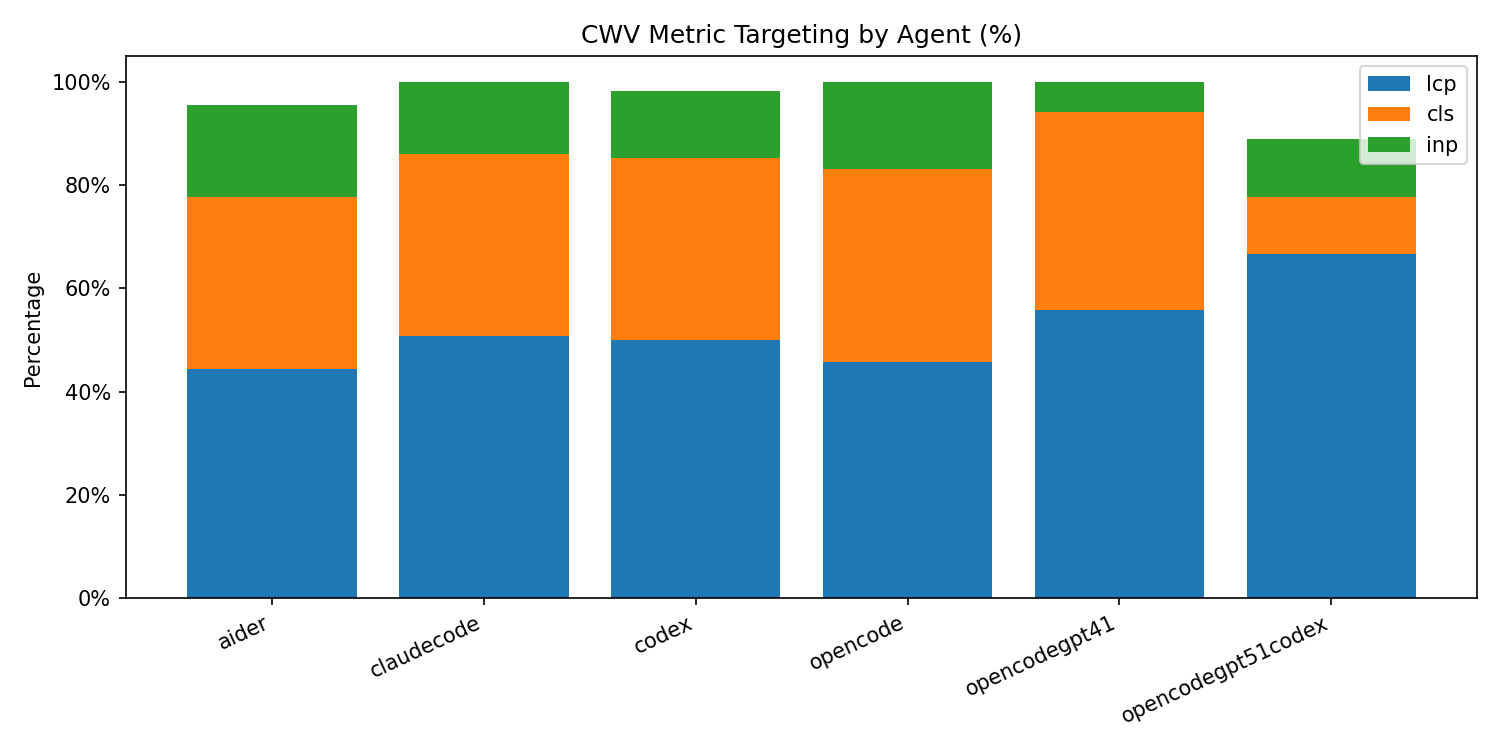
\includegraphics[width=0.8\linewidth]{figures/fig14_cwv_metric_target_stacked_by_agent.png}
    \caption{CWV metric targeting distribution across agents.}
\end{figure}

Across all agents, LCP dominates as the primary optimization target, with CLS receiving moderate attention and INP consistently underrepresented. This imbalance reflects a systematic bias toward load-time improvements over interaction latency, despite the growing importance of INP in modern CWV evaluation.

\subsubsection{CWV Metrics vs.\ Cost (Scatter Plot)}
\begin{figure}[t]
    \centering
    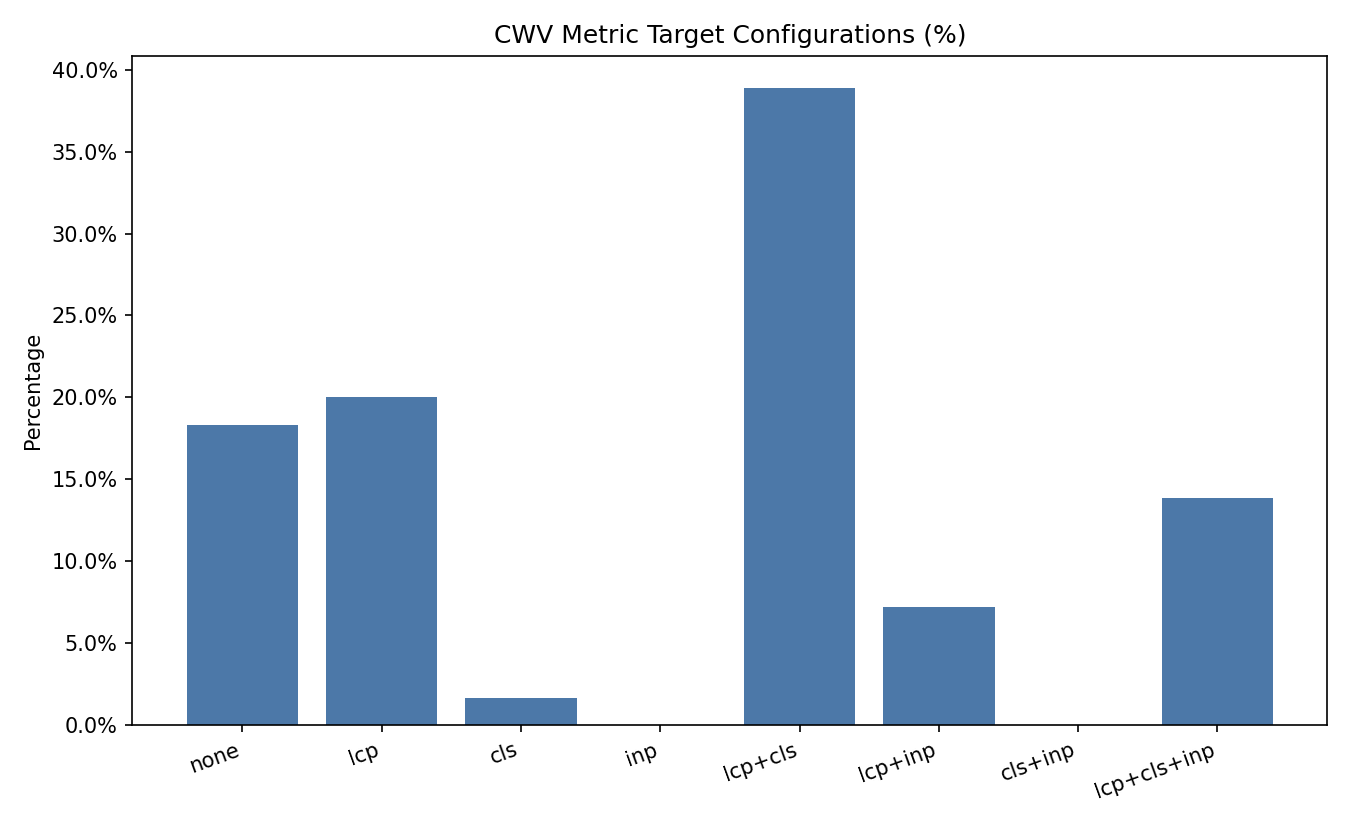
\includegraphics[width=0.7\linewidth]{figures/fig16_cwv_metric_pair_cooccurrence.png}
    \caption{CWV Improvement targets combined distribution}
    \label{fig:cost_tokens}
\end{figure}

% 3
\subsection{What broad techniques does the Agent try and use to achieve it's goals?}
\begin{figure}[t]
    \centering
    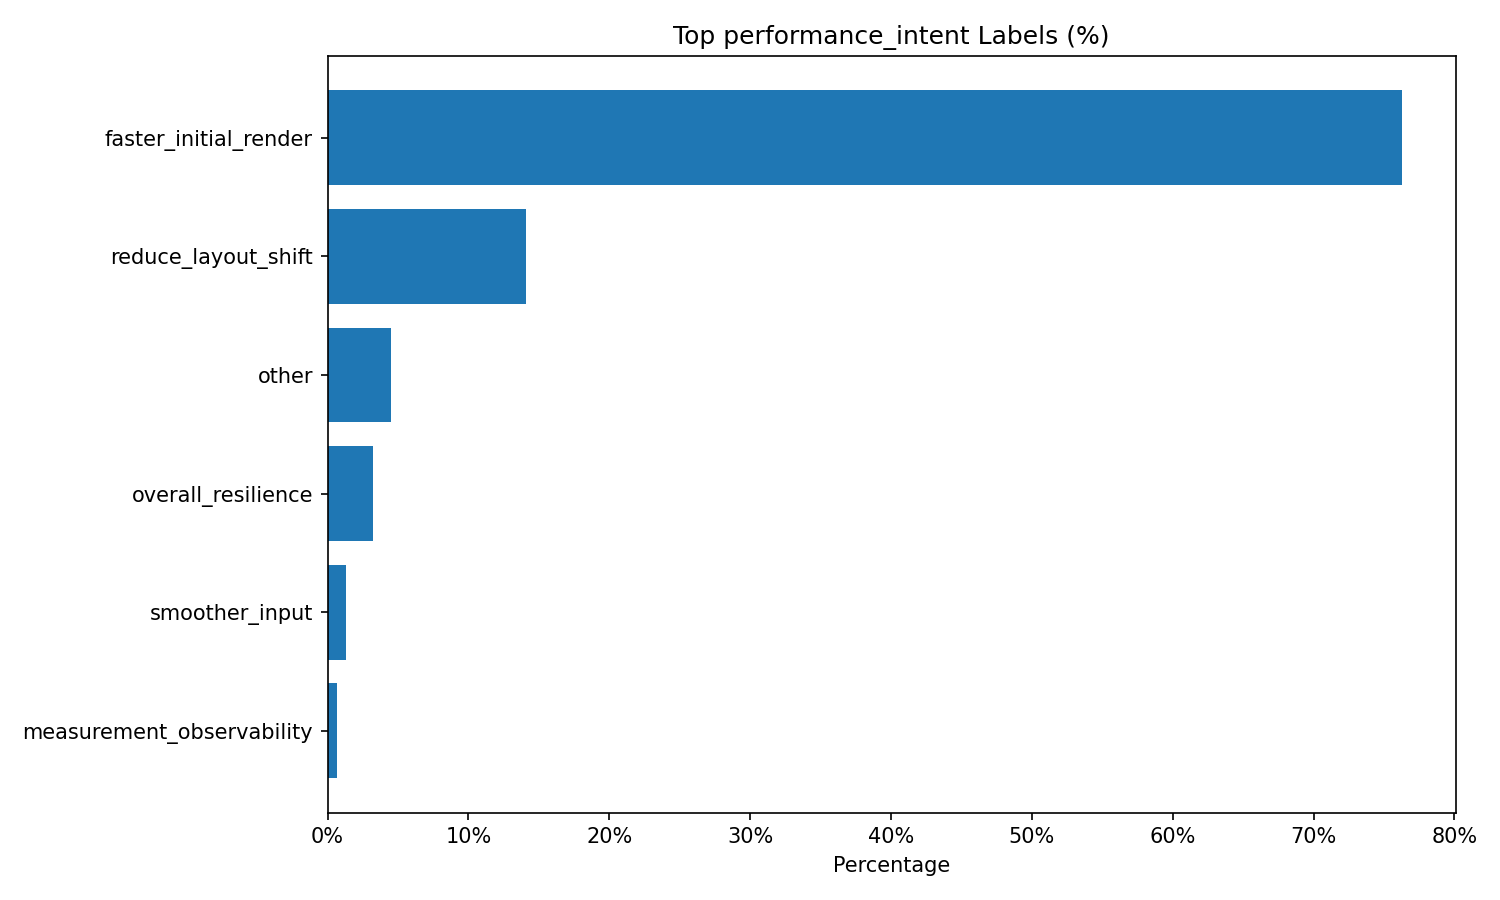
\includegraphics[width=0.8\linewidth]{figures/fig06_top_intent_labels.png}
    \caption{Top performance intent labels.}
\end{figure}

\begin{figure}[t]
    \centering
    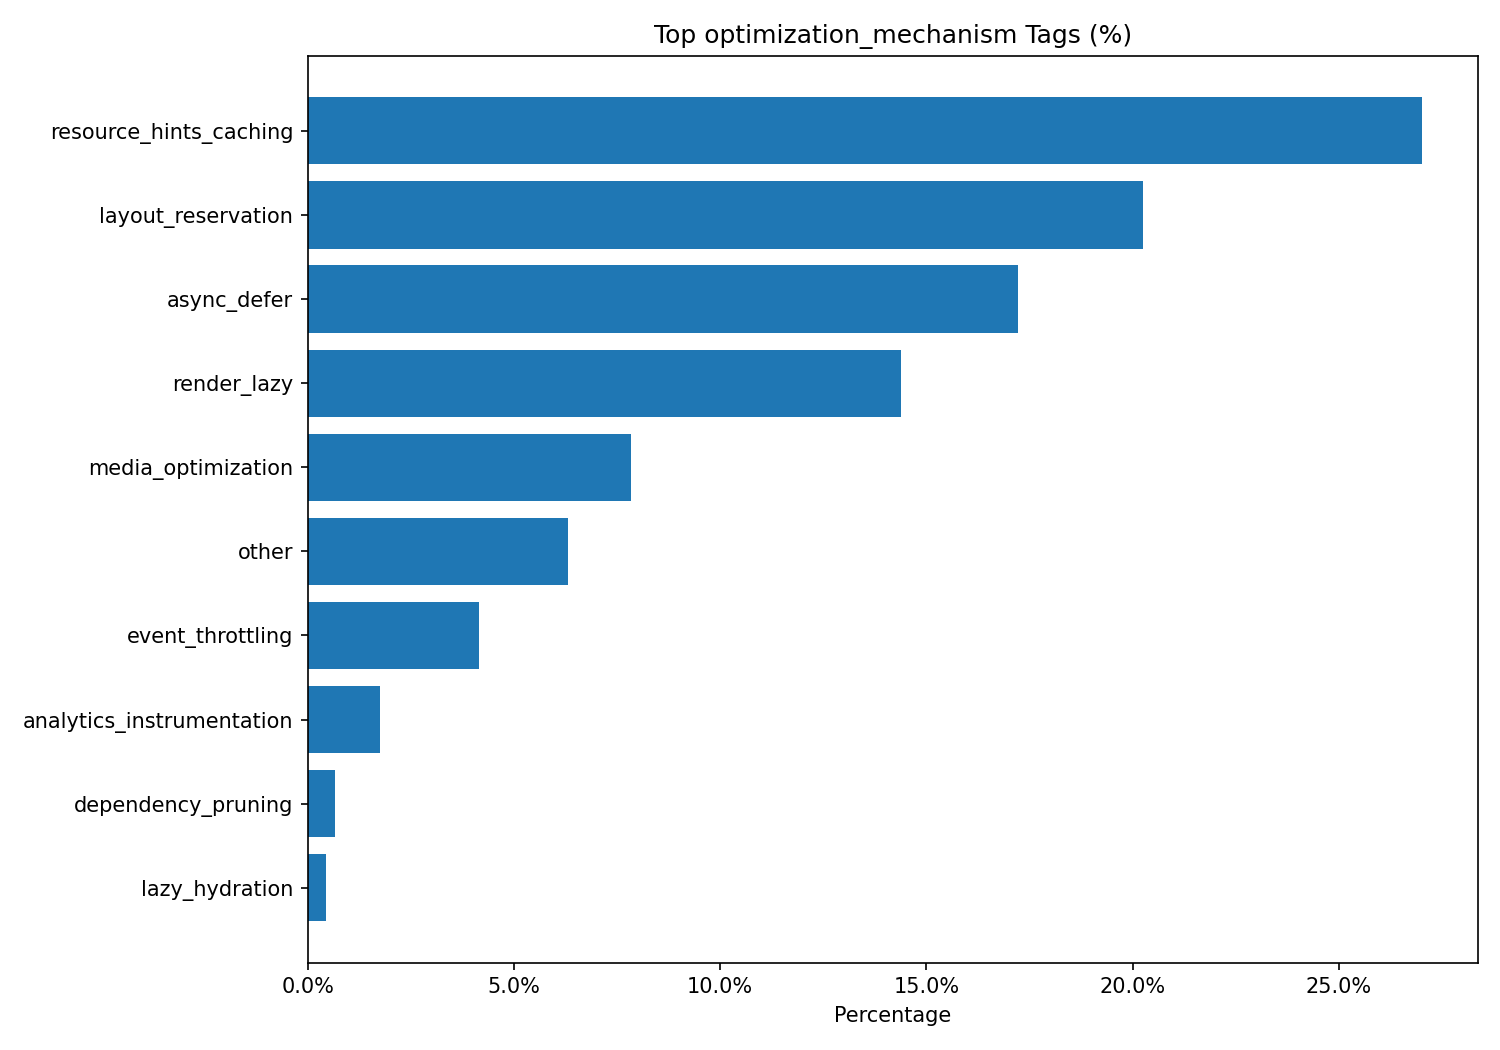
\includegraphics[width=0.8\linewidth]{figures/fig07_top_techniques.png}
    \caption{Top optimization mechanisms.}
\end{figure}

\begin{figure}[t]
    \centering
    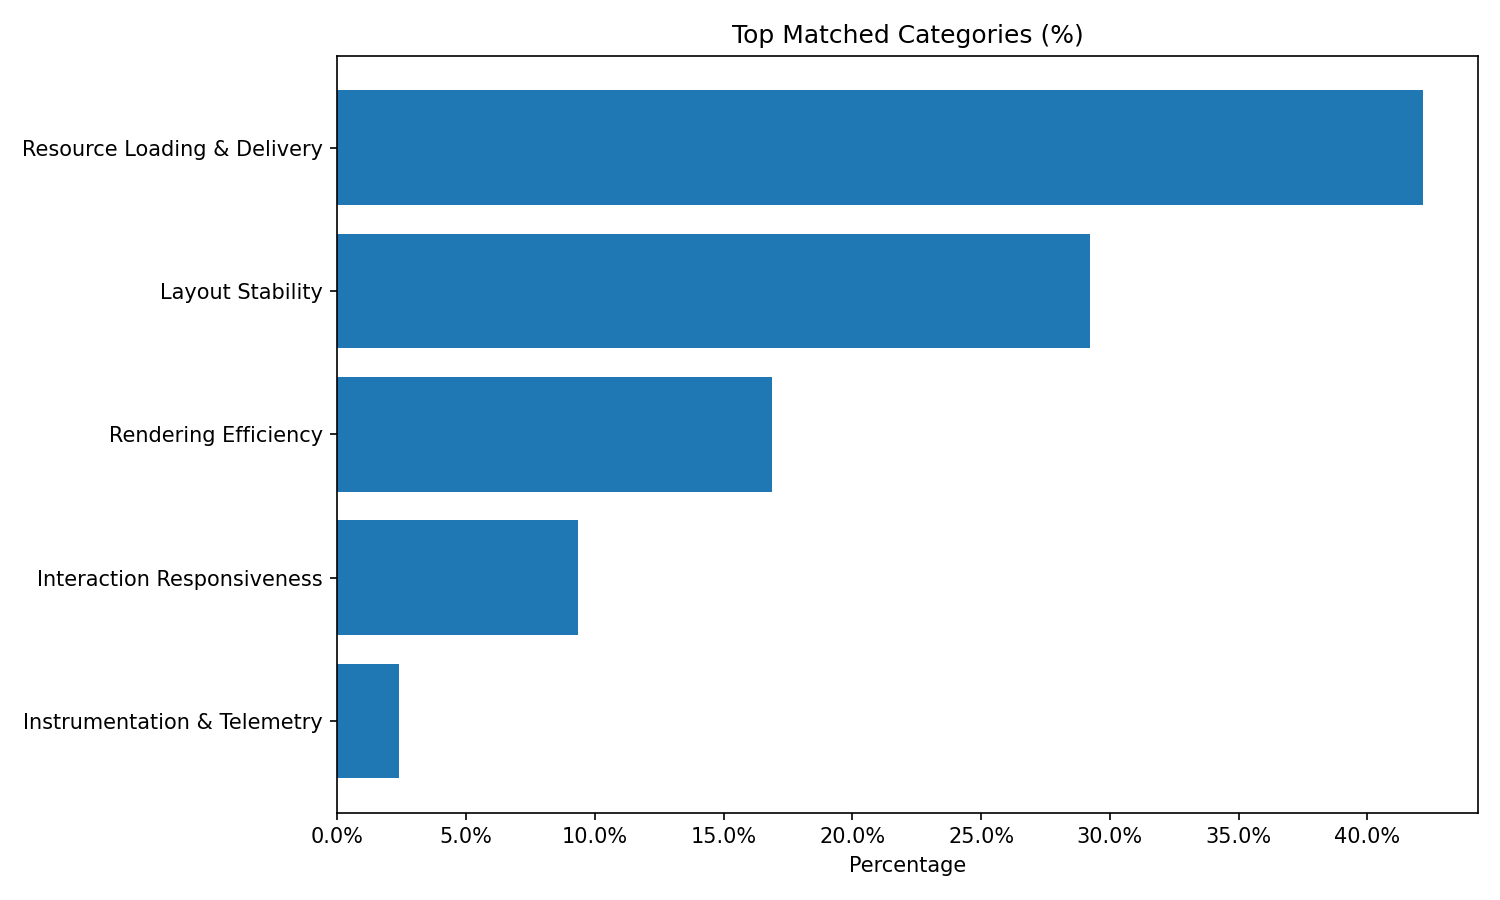
\includegraphics[width=0.8\linewidth]{figures/fig05_top_categories.png}
    \caption{Top matched optimization categories.}
\end{figure}

\begin{figure}[t]
    \centering
    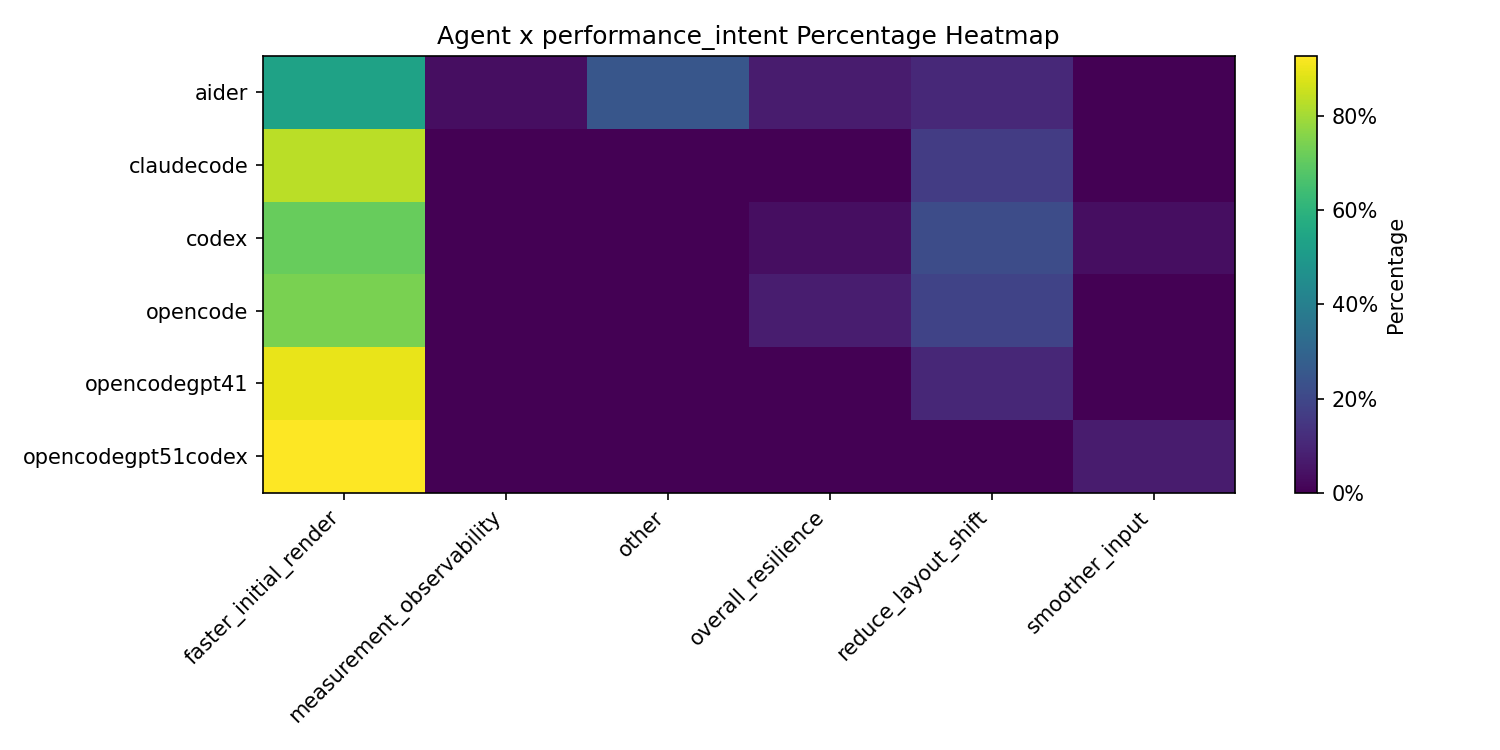
\includegraphics[width=0.8\linewidth]{figures/fig12_agent_intent_heatmap.png}
    \caption{Agent vs performance intent distribution.}
\end{figure}

\begin{figure}[t]
    \centering
    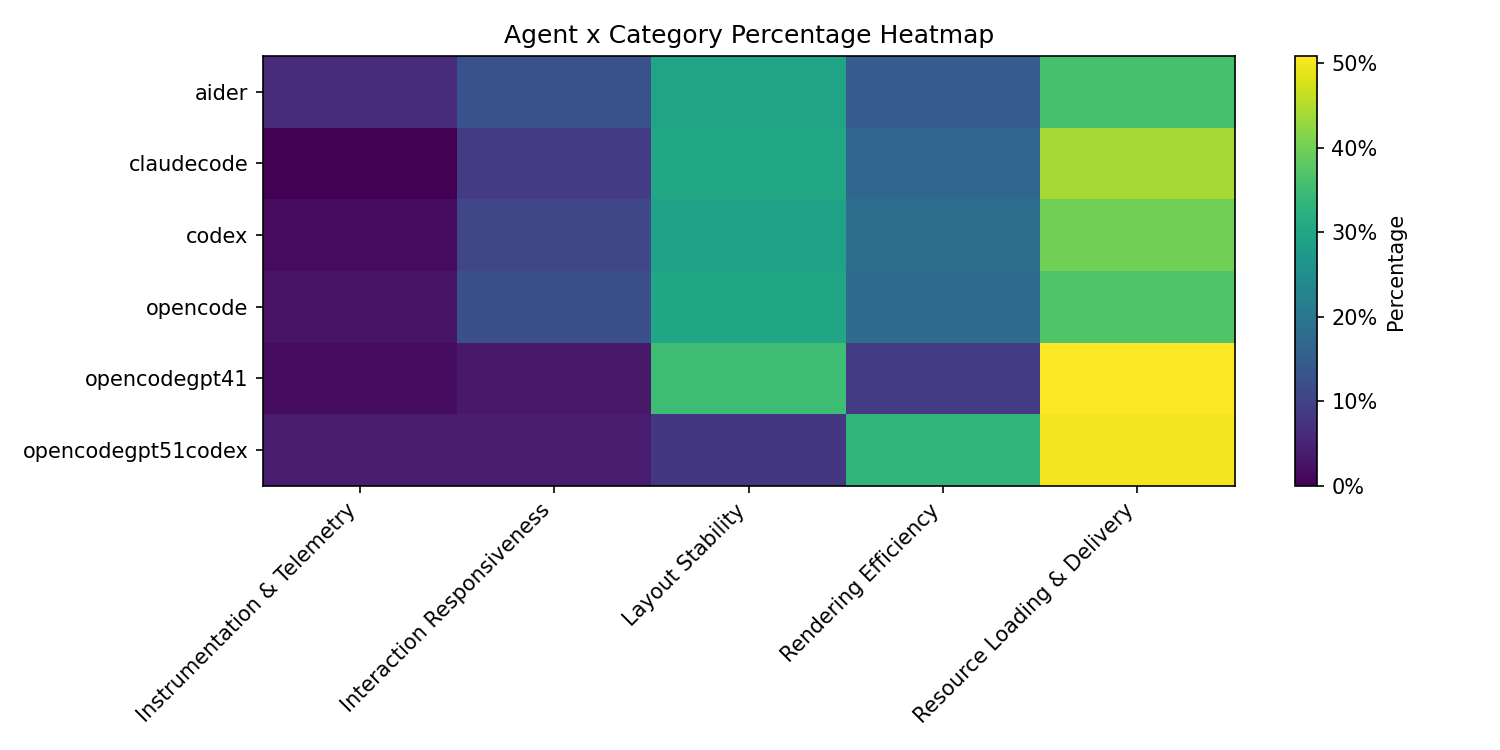
\includegraphics[width=0.8\linewidth]{figures/fig11_agent_category_heatmap.png}
    \caption{Agent vs optimization category distribution.}
\end{figure}

% 4
\subsection{How risky are the changes made by the agent in terms of harming the codebase as whole?}
\begin{figure}[t]
    \centering
    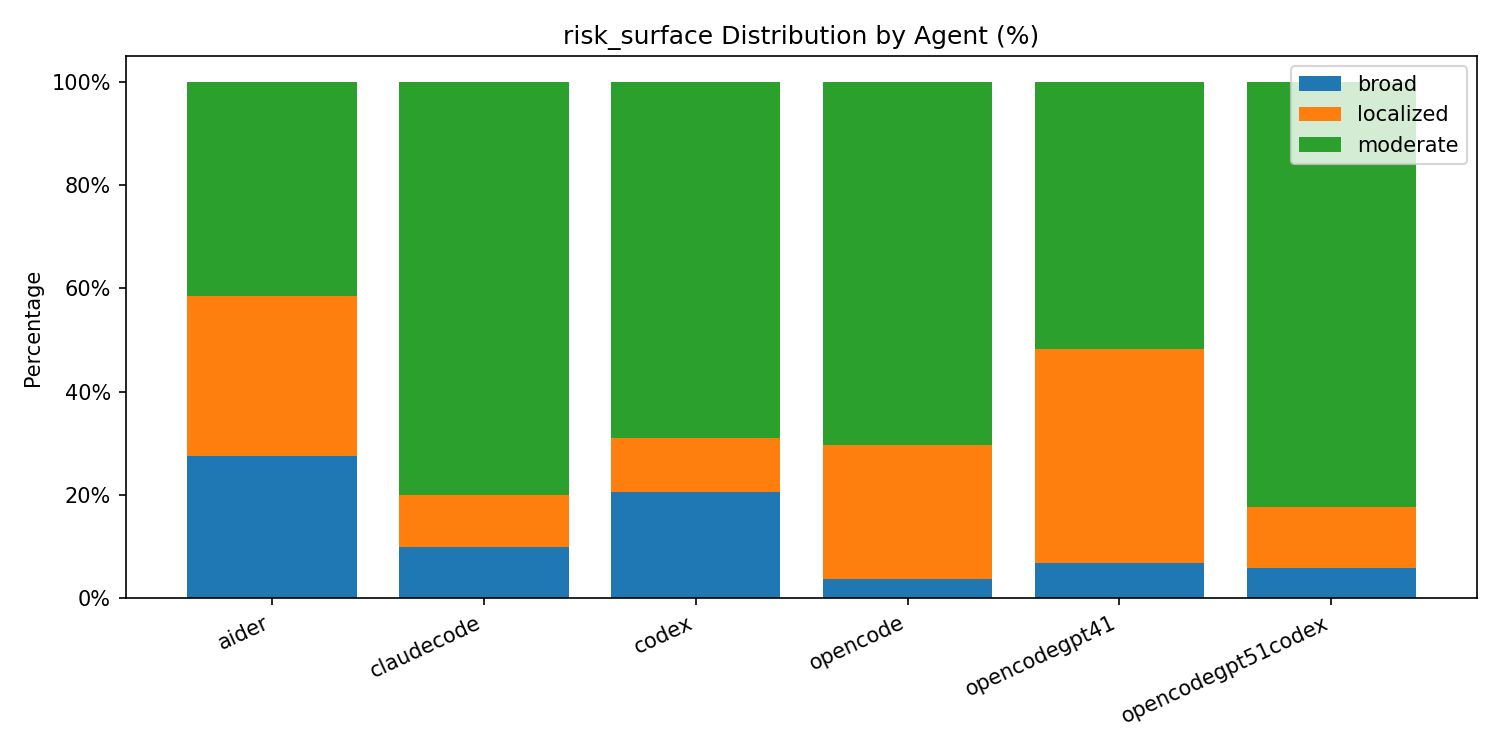
\includegraphics[width=0.8\linewidth]{figures/fig08_risk_stacked_by_agent.png}
    \caption{Distribution of patch risk surface across agents.}
\end{figure}

% 5
\subsection{What are the trends in terms of Agents being good at specific Frameworks / Languages?}


% 6
\subsection{Which datapoints do the Agents find harder to solve; How do the agents compete with each other individually?}


% 7
\subsection{Are there any instances of Reward Hacking attempted by any Agent?}

We analyze patches for indications of reward hacking, defined as modifications that artificially improve reported metrics without delivering meaningful user-perceived gains. Overall, the prevalence appears low: 89.4\% of cases show no evidence (161/180), 8.9\% are marked as uncertain (16/180), 1.1\% exhibit weak signals (2/180), and only 0.6\% (1/180) is flagged as likely reward hacking.

The single high-confidence case (\texttt{opencodegpt51codex\_\_202.json}, confidence 0.72) involves deferring visible user interactions (e.g., variant or cart updates) using \texttt{requestIdleCallback}, which may artificially improve INP-style metrics while degrading real interaction responsiveness.

Two additional cases present weak signals upon manual inspection. One (\texttt{claudecode\_\_2726.json}) defers core initialization until after LCP, potentially biasing load-time metrics. Another (\texttt{opencodegpt41\_\_101.json}) enforces a global fixed image aspect ratio, which may reduce measured CLS without fully addressing underlying layout instability.

Notably, the majority of uncertain cases (12/16) are concentrated in the \texttt{opencodegpt51codex} agent. This uncertainty is primarily due to missing or incomplete patch diffs rather than clear evidence of suspicious behavior.

\subsection{Additional Change Categories Analysis}

As examples of relatively infrequent techniques, we observe:
\begin{itemize}
    \item defer\_simulation\_with\_requestIdleCallback
    \item use\_react\_purecomponent\_cells
    \item nav\_click\_delegation
    \item async\_yield\_before\_heavy\_task
    \item conditional\_backdrop\_filters
    \item React startTransition for tab switches
    \item startTransition defers non-urgent state work
    \item idle analytics loading
    \item custom non-blocking toast
    \item strip\_motion\_hooks
    \item inline hero stub
    \item responsive\_masonry\_init
    \item remove\_animation\_logic
\end{itemize}

